\section{\gotopins}

\begin{frame}
  \frametitle{What is \gotopins?}
  \begin{center}
    \gotopins processes a Go program to translate it to obtain a
    \textit{Kripke Structure} to apply \textbf{model checking}\cite{Alur2018}.\\
    Last June, we published a paper on \gotopins\cite{kirszenberg.21.spin},\
    a second one has been submitted.
  \end{center}
\end{frame}

\begin{frame}
  \frametitle{What is \gotopins?}
  \framesubtitle{Successive transformation}
  \begin{figure}[H]
    \centering
    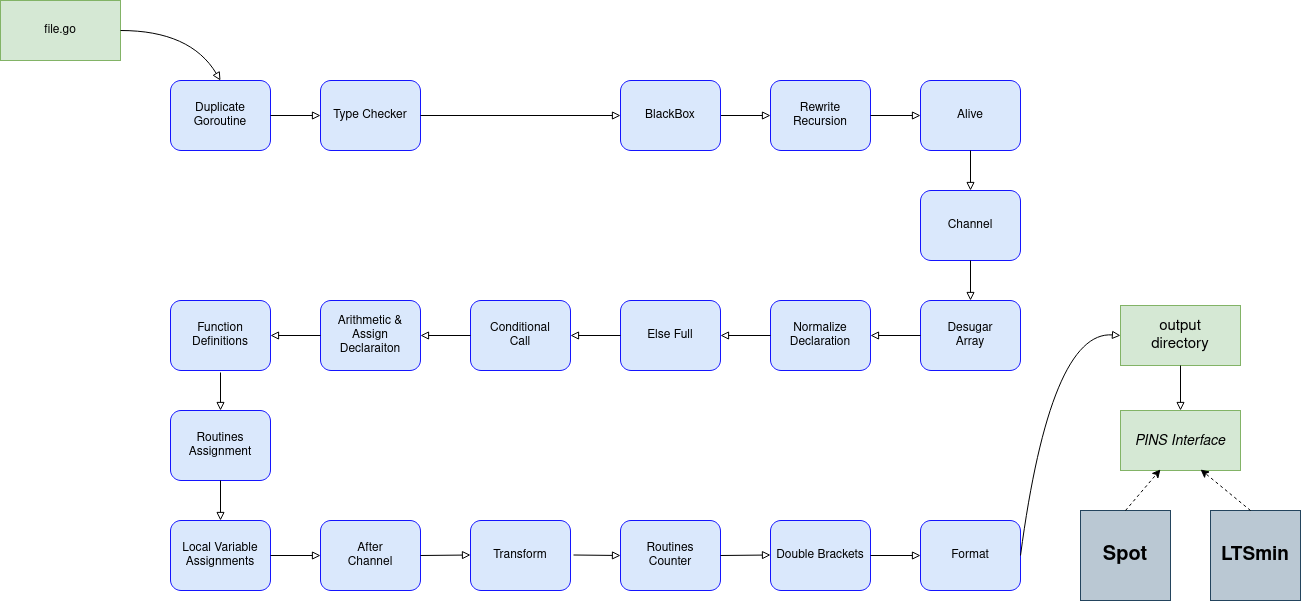
\includegraphics[width=11.8cm]{assets/TransformBeforeGlobal.png}
  \end{figure}
\end{frame}
